As shown on the Diagram, the system is composed of UserFrontEnd, 
AuthorityFrontEnd, ServerBackend, ReportDatabase, ViolationDatabase and 
CredentialDatabase.
Coherently with the pictures below, the development begins with the
definition of the schemas (one for each DB), this is known as 
Phase 0.
Phase 1 is composed of the development of the modules regarding the
exchange and management of data (Report Dispatcher, Info Dispatcher 
and Report Checker), as they provide the services central to Safestreets.
Phase 2 begins with the development of the modules and interfaces used 
for login and authentication (CheckManager and AuthenticationManager 
on the ServerBackend, AccessManager on UserFrontend and LoginManager on
AuthorityFrontEnd) while the integration of the external APIs is carried 
in parallel.
The last phase, labeled as 3, is dedicated to the completion of the 
FrontEnds, with the addition of the modules ReportManager and RequestManager.
The process is bottom-up as first the components to be developed 
first are the core ones, followed by those one who rely on their services,
and the testing is costant: every single unit is tested upon completion 
and then aggregate testing is carried out at the end of each phase to 
verify the ability of said components to cooperate.
Altough the focus is cast principally on functional testing , 
performance testing is used to measure and improve the throughput, still 
with the idea that the system does not have to be extremely fast to 
offer an optimal experience to users and authorities. Load and stress testing 
are also carried, to ensure availabilty even in critical conditions, 
such as the ones that can be found during rush hours in big cities.


\begin{figure}[H]
	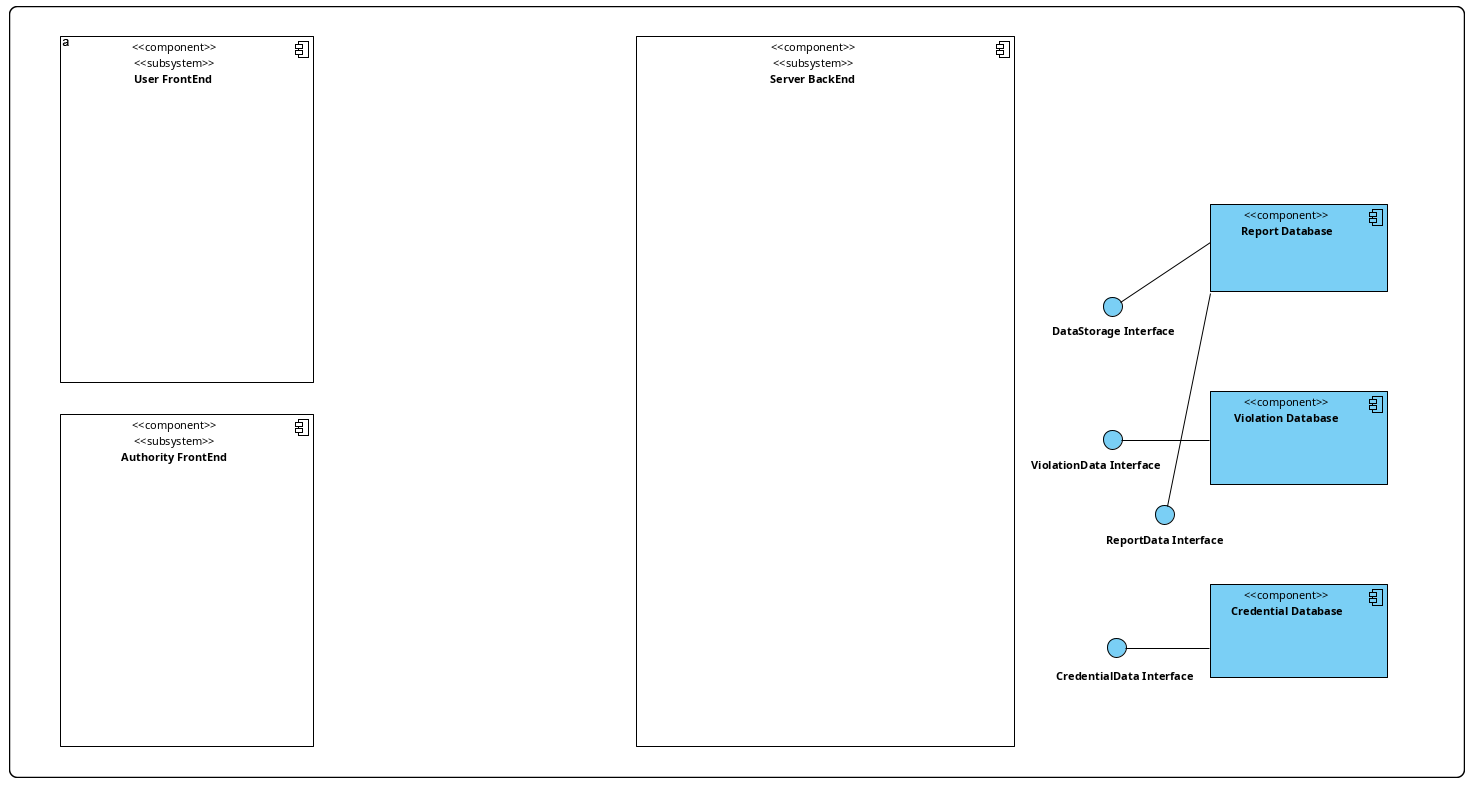
\includegraphics[width=\textwidth]{Images/ComponentView0.png}
	\caption{\label{fig:ComponentView0}Phase 0}
\end{figure}
\begin{figure}[H]
	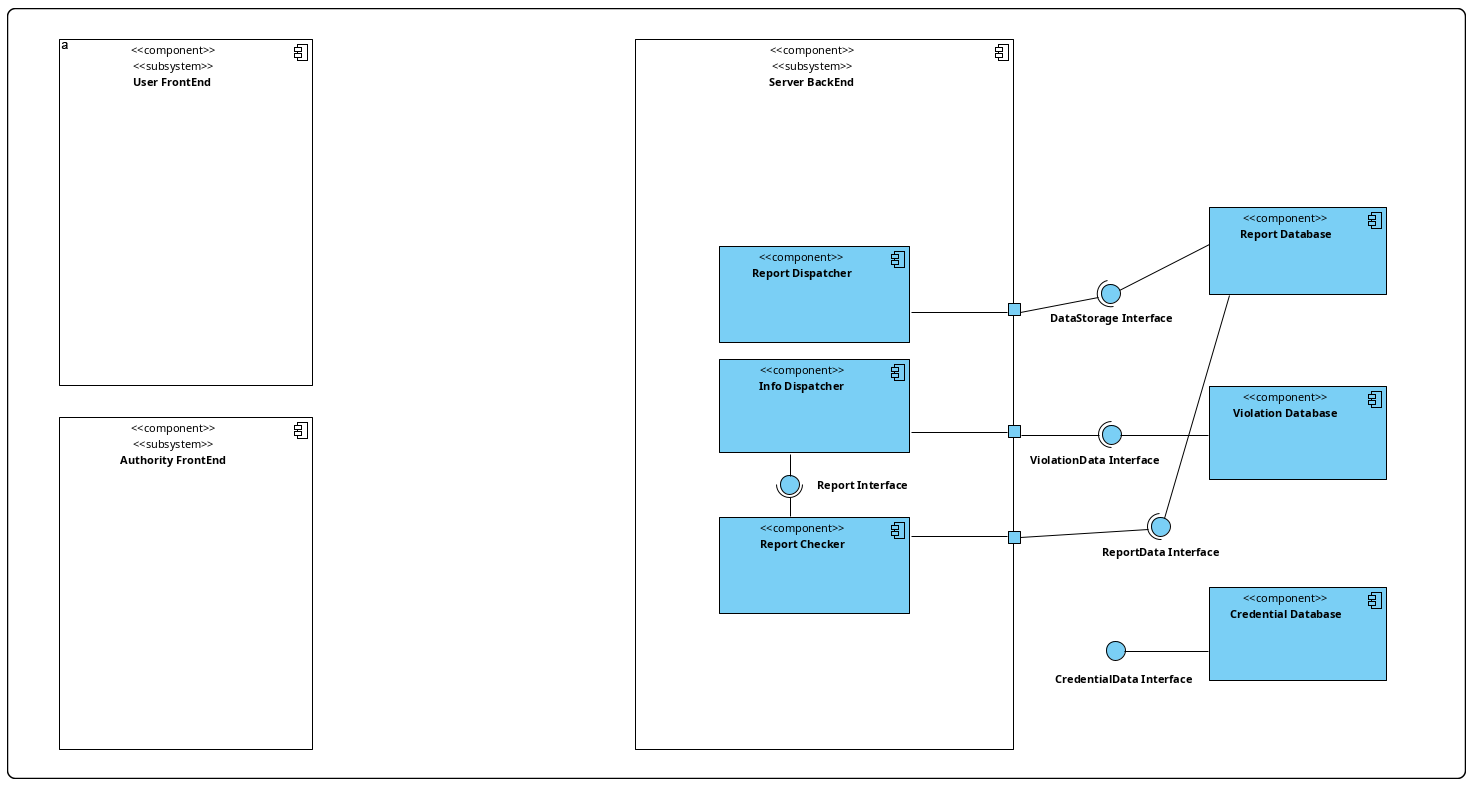
\includegraphics[width=\textwidth]{Images/ComponentView1.png}
	\caption{\label{fig:ComponentView1}Phase 1}
\end{figure}
\begin{figure}[H]
	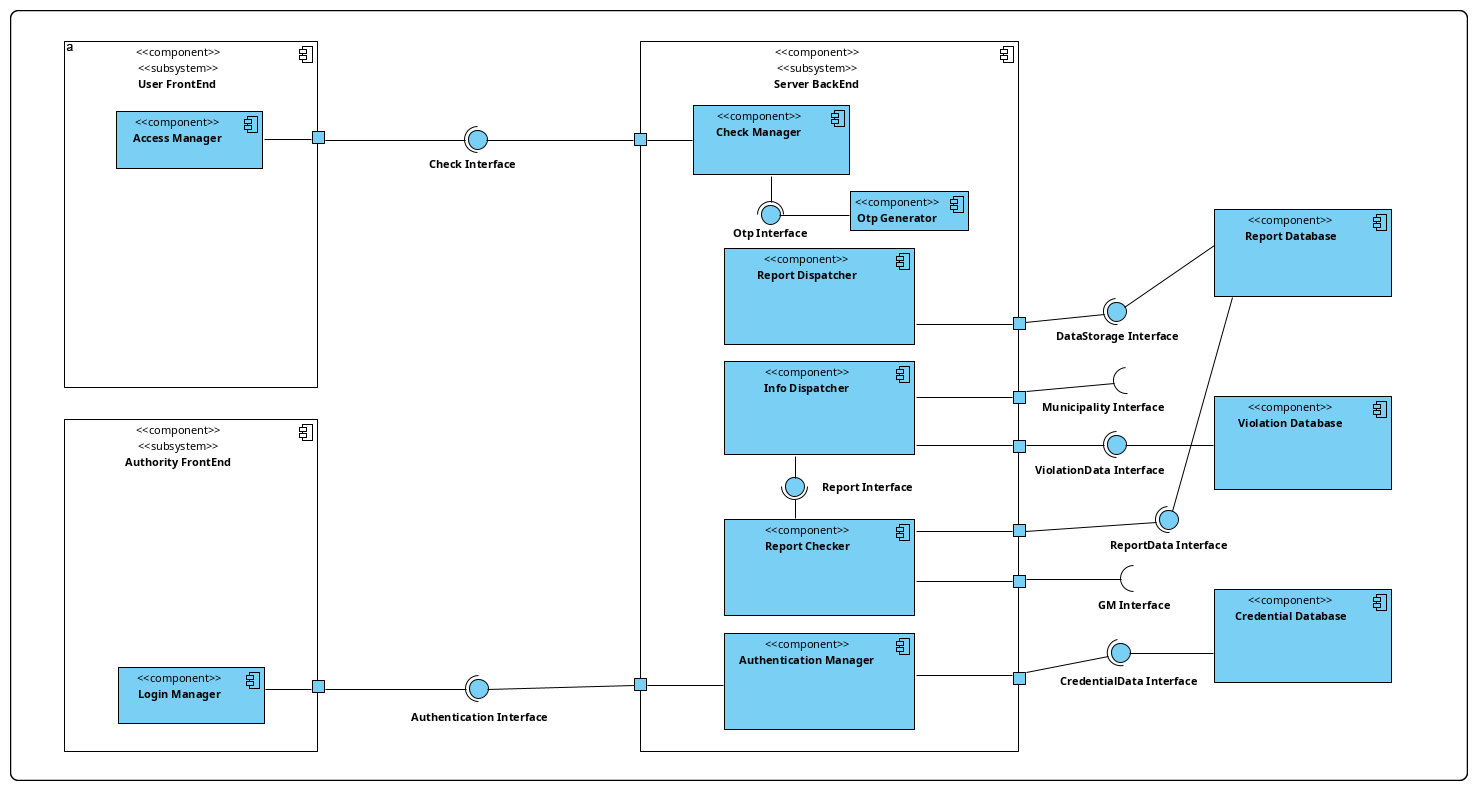
\includegraphics[width=\textwidth]{Images/ComponentView2.png}
	\caption{\label{fig:ComponentView2}Phase 2}
\end{figure}
\begin{figure}[H]
	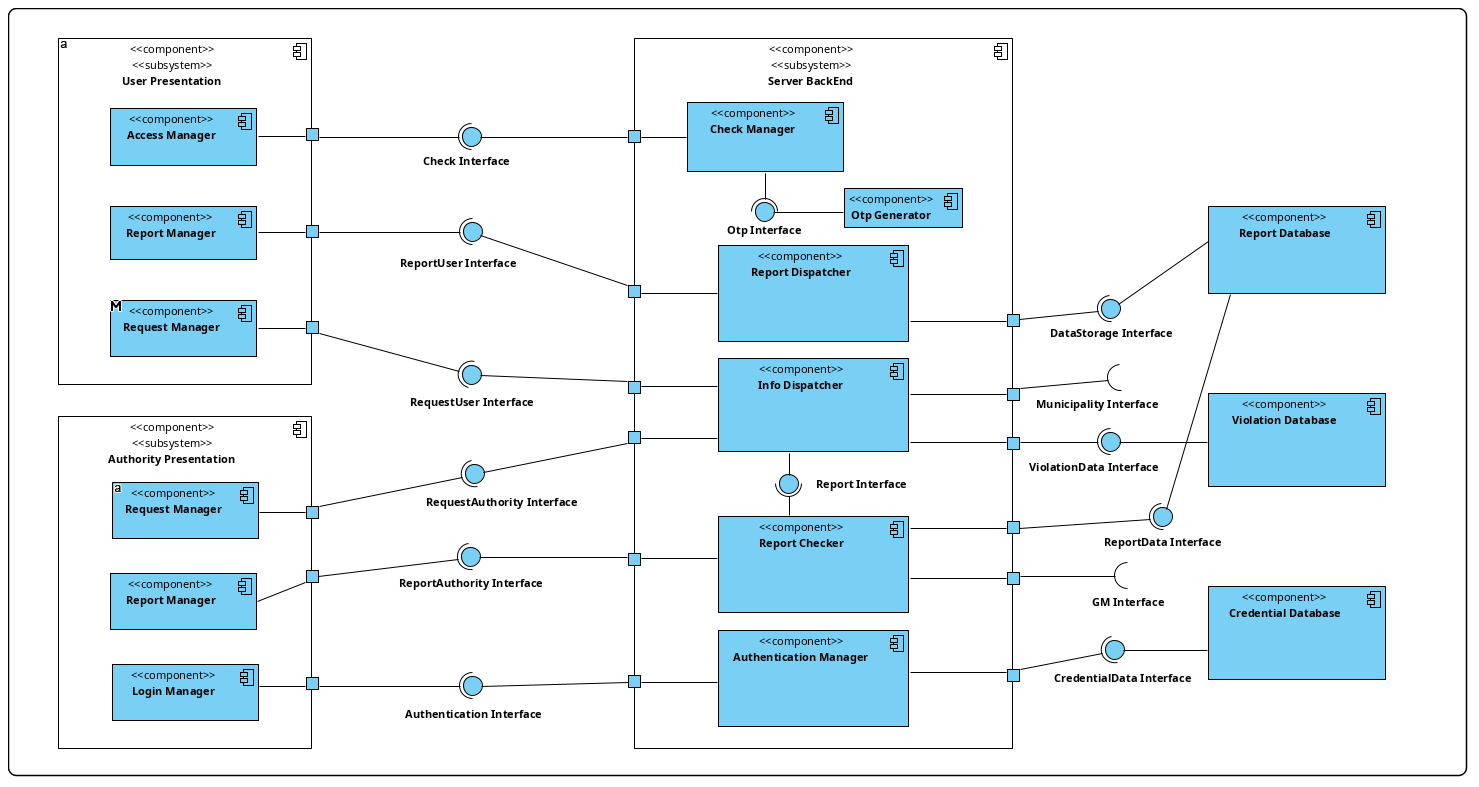
\includegraphics[width=\textwidth]{Images/ComponentView3.png}
	\caption{\label{fig:ComponentView3}Phase 3}
\end{figure}